\documentclass[]{article}
\usepackage{polski}
\usepackage{graphicx}
\usepackage{xcolor}
\usepackage{subcaption}
\usepackage{geometry}
\usepackage{ragged2e}
\usepackage{amsthm}
\usepackage{amsmath}
\usepackage{amssymb}
\usepackage{titlesec}
\usepackage{float}
\usepackage{etoolbox}
\usepackage{hyperref}
\usepackage{fancyhdr}
\usepackage{biblatex}
\geometry{
	a4paper,
	left=2.5cm,
	right=2.5cm,
	top=3cm,
	bottom=3cm}
\titleformat{\section}[hang]{\LARGE\bfseries\raggedright}{\thesection}{0.5cm}{}
\titleformat{\subsection}[hang]{\large\bfseries\raggedright}{\thesubsection}{0.5cm}{}
\newtheorem*{df}{\textcolor{red}{DEFINICJA}}
\newtheorem*{tw}{\textcolor{blue}{TWIERDZENIE}}
\begin{document}
	

	
	\begin{center}
		\centering
		\vspace*{2cm}
		
		\textbf{\Huge  POLITECHNIKA LUBELSKA} \\
		\vspace{0.5cm}
		\textbf{\LARGE WYDZIAŁ MATEMATYKI I} \\
		\vspace{0.5cm}
		\textbf{\LARGE INFORMATYKI TECHNICZNEJ}\\
		\vspace{1cm}
		
		\textit{Kierunek:} Inżynieria i Analiza Danych \\
		
		
		
		
	\end{center}
	
	
	\begin{figure}[h]
		
\includegraphics[width=0.4\textwidth]{logo_politechniki.png}
		\label{}
		\centering
	\end{figure}
	\begin{figure}[h]
		
\includegraphics[width=0.4\textwidth]{logo_wydziału}
		\label{}
		\centering
	\end{figure}
	\centering
	\textbf{Narzędzia informatyczne II}\\
	\vspace{0.5cm}
	\centering
	\textbf{Projekt zaliczeniowy Maxima}\\
	\vspace{0.5cm}
	
	\textit{Wykonała } \textbf{Maja Darczuk}
	
	\newpage
	
	\section*{\textbf{\Huge Badanie przebiegu zmienności funkcji}}
	
	\tableofcontents
	\section{Badanie funkcji $f(x)=\frac{e^{x}}{x}$}
	\begin{FlushLeft}
	Na wstepie zdefiniujmy funkcje w programie
	\end{FlushLeft}
	\begin{verbatim}
			/* Definicja funkcji */
			f(x) := (%e^x)/x$;
			print("Funkcja: ",f(x))$;
	\end{verbatim}
	\begin{figure}[H]
		\begin{flushleft}
		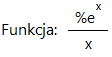
\includegraphics[width=0.15\linewidth]{zdj1}
		\end{flushleft}
	\end{figure}
	\subsection{Dziedzina}
	\begin{FlushLeft}
		\textbf{Dziedziną} funkcji jest $D=\mathbb{R}\setminus \{0\}$.
		\begin{verbatim}
			/* Obliczanie dziedziny */
			Dziedzina: solve([denom(f(x)) != 0], x)$;
			print("Dziedzina: ",Dziedzina)$;
		\end{verbatim}
		\begin{figure}[H]
			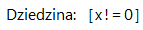
\includegraphics[width=0.17\linewidth]{zdj9}
		\end{figure}
	\end{FlushLeft}
	\newpage
	\subsection{Asymptoty}
	\begin{FlushLeft}
		\textbf{Asymptota pionowa } istnieje ponieważ funckja ma mianownik, który dla  $x=0$ dąży do nieskończoności, zatem istnieje asymptota pionowa w tym punkcie.
		\begin{verbatim}
			/* Asymptota pionowa */
			asymptota_pionowa_plus : limit(f(x), x, 0, plus)$;
			print("Granica dla x -> 0 z prawej: ", asymptota_pionowa_plus)$;
			
			asymptota_pionowa_minus : limit(f(x), x, 0, minus)$;
			print("Granica dla x -> 0 z lewej: ", asymptota_pionowa_minus)$;
		\end{verbatim}	
		\begin{figure}[H]
			\begin{flushleft}
				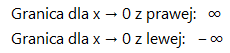
\includegraphics[width=0.3\linewidth]{zdj5}
			\end{flushleft}
		\end{figure}
		\textbf{Asymptota pozioma } nie istnieje ponieważ dla $ x \to + \infty $ funkcja dąży do $\infty$, a dla $ x \to - \infty $ funckja dąży do 0.
		\begin{verbatim}
			/* Asymptota pozioma */
			asymptota_pozioma_plus_inf : limit(f(x), x, inf)$;
			print("Granica dla x -> +inf: ", asymptota_pozioma_plus_inf)$;
			
			asymptota_pozioma_minus_inf : limit(f(x), x, minf)$;
			print("Granica dla x -> -inf: ", asymptota_pozioma_minus_inf)$;
		\end{verbatim}
		\begin{figure}[H]
			\begin{flushleft}
				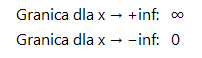
\includegraphics[width=0.25\linewidth]{zdj6}
			\end{flushleft}
		\end{figure}
		\textbf{Asymptota ukośna } nie istnieje.
		\begin{verbatim}
			/* Obliczenie współczynnika a */
			a : limit(f(x)/x, x, inf)$;
			print("Współczynnika a asymptoty ukośnej: ", a)$;
			
			/* Obliczenie współczynnika b */
			b : limit(f(x) - a * x, x, inf)$;
			print("Współczynnika b asymptoty ukośnej: ", b)$;
			print("Równanie asymptoty ukośnej: y = ", a, "* x + ", b)$;
			/*Zatem widać, że nie istnieje asymptota ukośna*/
		\end{verbatim}
		\begin{figure}[H]
			\begin{flushleft}
				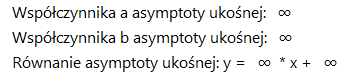
\includegraphics[width=0.5\linewidth]{zdj7}
			\end{flushleft}
		\end{figure}
	\end{FlushLeft}
	\newpage

	
	\subsection{Miejsce zerowe}
	\begin{FlushLeft}
		\textbf{Miejsce zerowe} nie istnieje.
		\begin{verbatim}
			/* Obliczenie miejsca zerowego funkcji */
			Miejsce_zerowe : solve(f(x) = 0, x)$;
			print("Miejscem zerowym funkcji jest: ",Miejsce_zerowe)$;
		\end{verbatim}
		\begin{figure}[H]
			\begin{flushleft}
				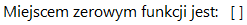
\includegraphics[width=0.35\linewidth]{zdj2}
			\end{flushleft}
		\end{figure}
	
	\end{FlushLeft}
	\subsection{Znaki funkcji}
	\begin{FlushLeft}
		Funkcja jest \textbf{dodatnia } dla $x > 0$, ponieważ  $e^{x}>0$ oraz $x>0$ zatem $\frac{e^{x}}{x}>0$.
		Funkcja jest \textbf{ujemna } dla $x > 0$, ponieważ $e^{x}>0$ oraz $x<0$ zatem $\frac{e^{x}}{x}<0$.
		\begin{verbatim}
			/*Sprawdzanie znaku funkcji*/
			Nierownosc_licznik_wiekszy_od_zera: %e^x>0$;
			print("Czy nierówność",Nierownosc_licznik_wiekszy_od_zera," jest prawdziwa?")$;
			Czy_prawdziwa:is(Nierownosc_licznik_wiekszy_od_zera)$;
			print(Czy_prawdziwa)$;
			print("Sprawdziliśmy, że ",Nierownosc_licznik_wiekszy_od_zera," jest
			prawdziwa zatem znak funkcji zależy od znaku x")$;
		\end{verbatim}
		\begin{figure}[H]
			\begin{flushleft}
				
\includegraphics[width=0.8\linewidth]{zdj8}
			\end{flushleft}
		\end{figure}
	\end{FlushLeft}
	\subsection{Pochodna funkcji}
	\begin{FlushLeft}
		\textbf{Pochodna} funkcji $f(x)=\frac{e^{x}}{x}$ wynosi 
		$ f'(x) = \frac{e^x}{x} - \frac{e^x}{x^2}$.
		\begin{verbatim}
		/* Obliczenie pochodnej */
		df : diff(f(x), x)$;
		print("Pochodna funkcji jest równa f'(x)= ",df)$;
		\end{verbatim}
		
		\begin{figure}[H]
			\begin{flushleft}
				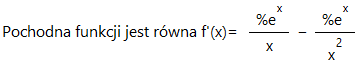
\includegraphics[width=0.5\linewidth]{zdj3}
			\end{flushleft}
		\end{figure}
	\end{FlushLeft}
	\newpage
	\subsection{Extrema lokalne}
	\begin{FlushLeft}
		Funkcja ma extremum lokalne minimalne w $x=1$ o wartości $f(1)=e$.
	
	\begin{verbatim}
	  /* Znalezienie miejsc zerowych pochodnej (potencjalne ekstremum) */
	punkt_extremum : solve(df = 0, x)$;
	
	/* Wyodrębnienie wartości z równań */
	wartość_argumentu : map(rhs, punkt_extremum)$;
	
	/* Obliczenie wartości funkcji w potencjalnych ekstremach */
	wartosc_extremum : map(f, wartość_argumentu)$;
	
	/* Sprawdzanie rodzaju ekstremum w punktach krytycznych */
	for punkt in punkt_extremum do (
	x0 : rhs(punkt),
	if  at(df, x = x0 - 0.01) < 0 and at(df, x = x0 + 0.01) > 0 then(
	print("Punkt krytyczny x =", x0, "jest minimum lokalnym, f(x) =", 
	f(x),"i ma wartość y=",wartosc_extremum))
	else if at(df, x = x0 - 0.01) > 0 and at(df, x = x0 + 0.01) < 0 then (
	print("Punkt krytyczny x =", x0, "jest maksimum lokalnym, f(x) =", 
	f(x),"i ma wartość y=",wartosc_extremum)))$;
	\end{verbatim}
	\end{FlushLeft}
	\begin{figure}[H]
		\begin{flushleft}
			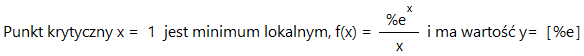
\includegraphics[width=0.8\linewidth]{zdj4}
		\end{flushleft}
	\end{figure}

	\subsection{Wykres}
	\begin{FlushLeft}
	
	\begin{verbatim}
		/* Tworzenie wykresu */
		draw2d(
		title = "Wykres funkcji f(x) = e^x/x i jej wlasnosci",
		xlabel = "x",
		ylabel = "y",
		
		/* Wykres funkcji f(x) linią niebieską */
		color = blue,
		key = "Funkcja f(x) = e^x/x",
		explicit(f(x), x, -5, 5),
		
		/* Punkt (1, e) czerwoną kropką jako ekstremum minimalne */
		color = red,
		point_type = filled_circle,
		key = "Ekstremum minimalne",
		points([[1, exp(1)]]),
		
		/* Linia przerywana zielona x = 0 */
		color = green,
		line_type = 2, /* Typ linii przerywana(2) */
		key = "Asymptota pionowa x = 0",
		implicit(x = 0, x, -5, 5, y, -10, 10), /* Rysowanie pionowej linii x = 0 */
		
		/* Wykres funkcji g(x) kropkowaną linią cyjanową jako pochodna */
		color = cyan,
		line_type = 3, /* Typ linii kropkowany(3) */
		key = "Pochodna df(x) = e^x*(x-1)/x^2",
		line_width = 1.5, /* Grubsza linia */
		explicit(df(x), x, -5, 5),
		
		/* Dodanie osi x i y */
		xaxis = true,
		yaxis = true,
		
		/* Ustawienie zakresów osi x i y */
		xrange = [-5, 5],
		yrange = [-10, 10]);
	\end{verbatim}
	\begin{figure}[H]
			\centering
			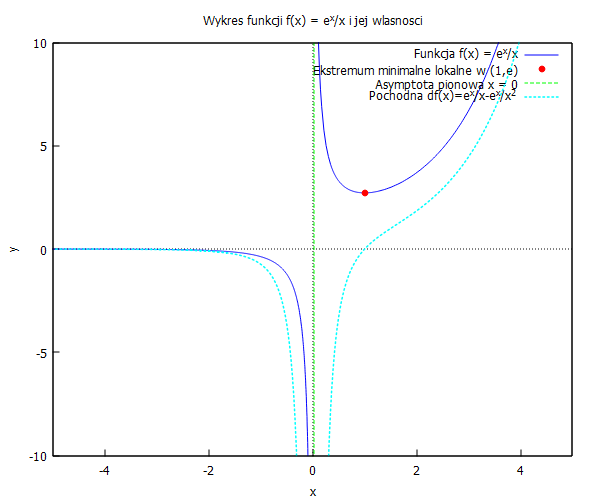
\includegraphics[width=0.7\linewidth]{Wykres_Funkcji}
	\end{figure}
	\end{FlushLeft}
	\subsection{Zbiór wartości}
	\begin{FlushLeft}
	\textbf{Zbiór wartości} określamy za pomocą wykresu ,granicy $\lim_{x \to -\infty} f(x)=0$ oraz extremum minimalnym lokalnym w punkcie $(1,e)$ otrzymując $ZW = (-\infty,0) \cup (e, \infty)$
	\end{FlushLeft}
	\subsection{Przedziały monotoniczności}
	\begin{FlushLeft}
	Wywołując wykres funkcji możemy odczytać jego przedziały monotoniczności. Funkcja jest \textbf{malejąca } dla $x \in (0,1)$.
	Funkcja jest \textbf{rosnąca } dla $x \in (-\infty,0) \cup (1, \infty)$.
	\end{FlushLeft}
	\newpage
	\section{Cały kod}
	\begin{verbatim}
		/* Definicja funkcji */
		f(x) := (%e^x)/x$;
		print("Funkcja: ",f(x))$;
		
		/* Obliczanie dziedziny */
		Dziedzina: solve([denom(f(x)) != 0], x)$;
		print("Dziedzina: ",Dziedzina)$;
		
		/* Asymptota pionowa */
		asymptota_pionowa_plus : limit(f(x), x, 0, plus)$;
		print("Granica dla x -> 0 z prawej: ", asymptota_pionowa_plus)$;
		
		asymptota_pionowa_minus : limit(f(x), x, 0, minus)$;
		print("Granica dla x -> 0 z lewej: ", asymptota_pionowa_minus)$;
		
		/* Asymptota pozioma */
		asymptota_pozioma_plus_inf : limit(f(x), x, inf)$;
		print("Granica dla x -> +inf: ", asymptota_pozioma_plus_inf)$;
		
		asymptota_pozioma_minus_inf : limit(f(x), x, minf)$;
		print("Granica dla x -> -inf: ", asymptota_pozioma_minus_inf)$;
		
		/*Asymptota ukośna*/
		/* Obliczenie współczynnika a */
		a : limit(f(x)/x, x, inf)$;
		print("Współczynnika a asymptoty ukośnej: ", a)$;
		
		/* Obliczenie współczynnika b */
		b : limit(f(x) - a * x, x, inf)$;
		print("Współczynnika b asymptoty ukośnej: ", b)$;
		print("Równanie asymptoty ukośnej: y = ", a, "* x + ", b)$;
		/*Zatem widać, że nie istnieje asymptota ukośna*/
		
		/* Obliczenie miejsca zerowego funkcji */
		Miejsce_zerowe : solve(f(x) = 0, x)$;
		print("Miejscem zerowym funkcji jest: ",Miejsce_zerowe)$;
		
		/*Sprawdzanie znaku funkcji*/
		Nierownosc_licznik_wiekszy_od_zera: %e^x>0$;
		print("Czy nierówność",Nierownosc_licznik_wiekszy_od_zera," jest prawdziwa?")$;
		Czy_prawdziwa:is(Nierownosc_licznik_wiekszy_od_zera)$;
		print(Czy_prawdziwa)$;
		print("Sprawdziliśmy, że ",Nierownosc_licznik_wiekszy_od_zera," jest
		prawdziwa zatem znak funkcji zależy od znaku x")$;
		
		/* Obliczenie pochodnej */
		df : diff(f(x), x)$;
		print("Pochodna funkcji jest równa f'(x)= ",df)$;
		
		/* Znalezienie miejsc zerowych pochodnej (potencjalne ekstremum) */
		punkt_extremum : solve(df = 0, x)$;
		
		/* Wyodrębnienie wartości z równań */
		wartość_argumentu : map(rhs, punkt_extremum)$;
		
		/* Obliczenie wartości funkcji w potencjalnych ekstremach */
		wartosc_extremum : map(f, wartość_argumentu)$;
		
		/* Sprawdzanie rodzaju ekstremum w punktach krytycznych */
		for punkt in punkt_extremum do (
		x0 : rhs(punkt),
		if  at(df, x = x0 - 0.01) < 0 and at(df, x = x0 + 0.01) > 0 then(
		print("Punkt krytyczny x =", x0, "jest minimum lokalnym, f(x) =",
		 f(x),"i ma wartość y=",wartosc_extremum))
		else if at(df, x = x0 - 0.01) > 0 and at(df, x = x0 + 0.01) < 0 then (
		print("Punkt krytyczny x =", x0, "jest maksimum lokalnym, f(x) =", 
		f(x),"i ma wartość y=",wartosc_extremum)))$;
		
		/* Tworzenie wykresu */
		draw2d(
		title = "Wykres funkcji f(x) = e^x/x i jej wlasnosci",
		xlabel = "x",
		ylabel = "y",
		
		/* Wykres funkcji f(x) linią niebieską */
		color = blue,
		key = "Funkcja f(x) = e^x/x",
		explicit(f(x), x, -5, 5),
		
		/* Punkt (1, e) czerwoną kropką jako ekstremum minimalne */
		color = red,
		point_type = filled_circle,
		key = "Ekstremum minimalne lokalne w (1,e)",
		points([[1, exp(1)]]),
		
		/* Linia przerywana zielona x = 0 */
		color = green,
		line_type = 2, /* Typ linii przerywana(2) */
		key = "Asymptota pionowa x = 0",
		implicit(x = 0, x, -5, 5, y, -10, 10), /* Rysowanie pionowej linii x = 0 */
		
		/* Wykres funkcji g(x) kropkowaną linią cyjanową jako pochodna */
		color = cyan,
		line_type = 3, /* Typ linii kropkowany(3) */
		key = "Pochodna df(x)=e^x/x-e^x/x^2 ",
		line_width = 1.5, /* Grubsza linia */
		explicit(df, x, -5, 5),
		
		/* Dodanie osi x i y */
		xaxis = true,
		yaxis = true,
		
		/* Ustawienie zakresów osi x i y */
		xrange = [-5, 5],
		yrange = [-10, 10]);
	\end{verbatim}

\section*{Źródła pomocnicze}
\patchcmd{\thebibliography}{\section*{\refname}}{}{}{}
\begin{thebibliography}*{}
$\bullet$  Prezentacje Wykładu "Narzędzia Informatyczne II" dr inż. Anny Futy
	
	
\end{thebibliography}
\end{document}